\section{Perceptron}

Neste problema, você criará a sua própria função target $f$ e uma base de dados $D$ para que possa ver como o
Algoritmo de Aprendizagem Perceptron funciona. Escolha $d = 2$ pra que você possa visualizar o problema,
e assuma $\chi = [-1, 1] \times [-1, 1]$ com probabilidade uniforme de escolher cada $x \in \mathcal{X}$ .

Em cada execução, escolha uma reta aleatória no plano como sua função target $f$ (faça isso selecionando dois pontos aleatórios, uniformemente distribuídos em  $\chi = [-1, 1] \times [-1, 1]$, e pegando a reta que passa entre eles), de modo que um lado da reta mapeia pra +1 e o outro pra -1. Escolha os inputs $x_n$ da base de dados como um conjunto de pontos aleatórios (uniformemente em $ \mathcal{X}$ ), e avalie a função target em cada $x_n$ para pegar o output correspondente $y_n$.

Agora, pra cada execução, use o Algoritmo de Aprendizagem Perceptron (PLA) para encontrar $g$. Inicie o PLA com um vetor de pesos $w$ zerado (considere que $sign(0) = 0$, de modo que todos os pontos estejam classificados erroneamente ao início), e a cada iteração faça com que o algoritmo escolha um ponto aleatório dentre os classificados erroneamente. Estamos interessados em duas quantidades: o número de iterações que o PLA demora para convergir pra $g$, e a divergência entre $f$ e $g$ que é $\mathbb{P}[f (x) \neq g(x)]$ (a probabilidade de que $f$ e $g$ vão divergir na classificação de um ponto aleatório). Você pode calcular essa probabilidade de maneira exata, ou então aproximá-la ao gerar uma quantidade suficientemente grande de novos pontos para estimá-la (por exemplo, 10.000).

A fim de obter uma estimativa confiável para essas duas quantias, você deverá realizar 1000 execuções do experimento (cada execução do jeito descrito acima), tomando a média destas execuções como seu resultado
final.

Para ilustrar os resultados obtidos nos seus experimentos, acrescente ao seu relatório gráficos scatterplot
com os pontos utilizados para calcular $E_{out}$, assim como as retas correspondentes à função target e à hipótese $g$ encontrada.
\newline \par
\textbf{Implementação:}

Para responder os itens referentes a este problema, foi implementado em Python um Perceptron 2D utilizando as fórmulas e procedimentos apresentados na primeira aula do professor Yaser Abu-Mostafa. Foram criadas duas classes: uma para gerar a base de dados e a função target (código \ref{cod:database}) e outra pra criar e treinar o perceptron (código \ref{cod:perceptron}). Ambos os códigos estão listados abaixo.

\begin{lstlisting}[language=Python, caption=Geração do da base de dados $D$, label=cod:database]
    # Classe para criar o dataset e a função target
    class Dataset:
        def __init__(self, N): 
            self.N = N # tamanho do dataset
            self.a = 0 # coeficiente angular
            self.b = 0 # coeficiente linear
    
        # Método para gerar a linha da função target
        def generate_random_line(self):
            point1 = np.random.uniform(-1, 1, 2) # ponto aleatorio no domínio
            point2 = np.random.uniform(-1, 1, 2) # ponto aleatorio no domínio
            a = (point2[1] - point1[1]) / (point1[0] - point2[0]) # cálculo do coeficiente angular
            b = point1[1] - a*point1[0] # cálculo do coeficiente linear
            self.a = a
            self.b = b
            return a, b
    
        # Método para classificar pontos de acordo a função target
        def classify_point(self, point):
            a = self.a
            b = self.b
            y_reta = a*point[0] + b    
            return np.sign(point[1] - y_reta) # verifica se a coordenada y do ponto está acima ou abaixo da reta
    
        # Método para gerar a base de dados D
        def generate_dataset(self):
            N = self.N
            data = np.random.uniform(-1, 1, (N, 2)) # gera N pontos no R2 com coordenadas entre [-1, 1]
            labels = np.array([self.classify_point(point) for point in data])
            return data, labels
\end{lstlisting}

\begin{lstlisting}[language=Python, caption=Perceptron, label=cod:perceptron]
    # Classe para criar e treinar o perceptron 2D
    class Perceptron2D:
        def __init__(self, max_iter=1000):
            self.max_iter = max_iter
            self.w = np.zeros(3)  # inicializa os pesos (incluindo o w_0)
        
        # Método para treinar o perceptron usando o algoritmo de aprendizagem perceptron (PLA)
        def fit(self, data, labels): 
            n_samples = len(data)
            X_bias = np.hstack([np.ones((n_samples, 1)), data]) # adiciona uma coluna de 1s para o X_0 (coordenada artificial)
            iterations = 0
            errors = 1
            while (errors > 0) and (iterations <= self.max_iter):
                errors = 0
                for i in range(n_samples):
                    if labels[i] * np.dot(self.w, X_bias[i]) <= 0:
                        self.w += labels[i] * X_bias[i] # atualiza os pesos
                        errors += 1
                iterations += 1
            return iterations, self.w
        
        # Método para classificar um dataset com base nos pesos aprendidos.
        def classificar(self, data):
            n_samples = len(data)
            X_bias = np.hstack([np.ones((n_samples, 1)), data]) # adiciona uma coluna de 1s para o bias X_0
            return np.sign(np.dot(X_bias, self.w)) # verifica o sinal do produto escalar entre x e w
        
            # Método para plotar os resultados
        def plot(self, data, labels, a, b):
            plt.figure(figsize=(8, 6))
            x_pos = [data[i][0] for i in range(len(data)) if labels[i] == 1]
            y_pos = [data[i][1] for i in range(len(data)) if labels[i] == 1]
            x_neg = [data[i][0] for i in range(len(data)) if labels[i] == -1]
            y_neg = [data[i][1] for i in range(len(data)) if labels[i] == -1]
            plt.scatter(x_pos, y_pos, c='blue', label='+1')
            plt.scatter(x_neg, y_neg, c='red', label='-1')
            x = np.linspace(-1, 1, 100)
            y_target = a*x+b
            y_g = -(self.w[1] * x + self.w[0]) / self.w[2]
            plt.plot(x, y_g, 'g-', label='Hipótese (g)')
            plt.plot(x, y_target, 'k-', label='Função Target (f)')
            plt.xlim(-1, 1)
            plt.ylim(-1, 1)
            plt.xlabel('x')
            plt.ylabel('y')
            plt.title('Base de dados com o Target (f) e a Hipótese (g)')
            plt.legend(bbox_to_anchor=(1.05, 1), loc='upper left')
            plt.tight_layout(rect=[0, 0, 1, 1])
            plt.grid(True)
            plt.show()
\end{lstlisting}


Para testar as classes, foi feita uma função para plotar uma base de dados de 100 pontos com a função target $f$ gerada e a hipótese $g$ com a reta calculada pelo PLA (código \ref{cod:perceptron_teste}). O resultado pode ser observado na figura \ref{fig:perceptron_plot}. 

\begin{lstlisting}[language=Python, caption=Teste das classes, label=cod:perceptron_teste]
    def teste():
        num_points = 100
        pontos = Dataset(num_points)
        a, b = pontos.generate_random_line()
        data, labels = pontos.generate_dataset()
        perceptron = Perceptron2D()
        perceptron.fit(data,labels)
        perceptron.plot(data, labels, a, b)
\end{lstlisting}

\begin{figure}[H]
    \caption{Base de dados com o Target $(f)$ e a Hipótese $(g)$}
       \centering
       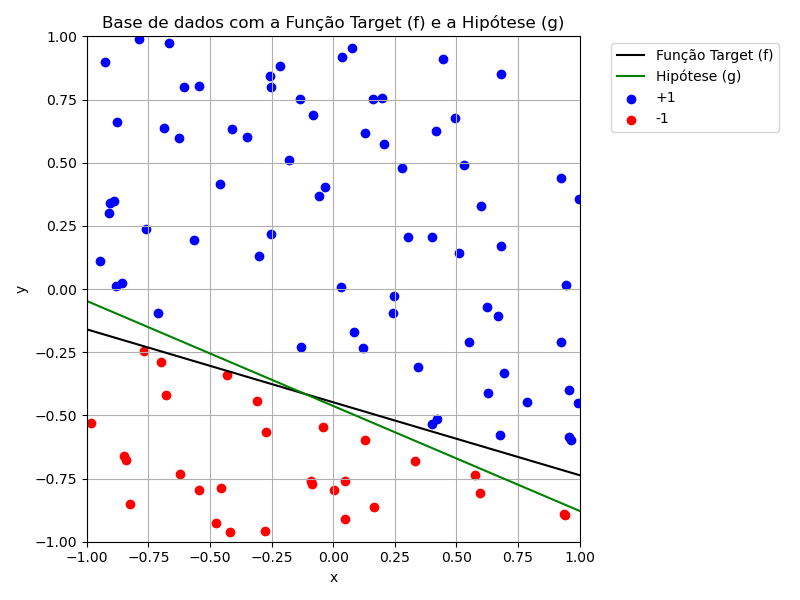
\includegraphics[height=8cm]{perceptron_plot.png}
    \label{fig:perceptron_plot}
\end{figure}



\begin{enumerate}
    \item Considere $N = 10$. Quantas iterações demora, em média, para que o PLA convirja com $N = 10$
    pontos de treinamento? Escolha o valor mais próximo do seu resultado.

    \begin{enumerate}
        \item[\textcolor{red}{(a)}]\textcolor{red}{1}\addtocounter{enumii}{1}
        \item 15
        \item 300
        \item 5000
        \item 10000
    \end{enumerate}
     
    \par

    \textbf{Justificativa:}

    Para responder a esse item foi implementada a seguinte função:

    \begin{lstlisting}[language=Python, caption=Item 1, label=cod:]
        def item_1():
        num_points = 10
        num_iter = list()
        for i in range(1000):
            pontos = Dataset(num_points)
            a, b = pontos.generate_random_line()
            data, labels = pontos.generate_dataset()
            perceptron = Perceptron2D()
            iter, _ = perceptron.fit(data,labels)
            num_iter.append(iter)
    
        print(f"item a) {np.mean(num_iter)} iterações com desvio padrão {np.std(num_iter):.4f} (min:{np.min(num_iter)}, máx:{np.max(num_iter)})"
    
    \end{lstlisting}

    O resultado após 1000 execuções do experimento foi uma média de $5,049(\approx 5)$ iterações, com desvio padrão de $7,777 (\approx 8)$ iterações, mínimo de 2 iterações e máximo de 99 iterações. Como 5 está mais próximo de 1 do que de 15, o \textcolor{red}{\textbf{item a}} foi selecionado. 
    
    \item Qual das alternativas seguintes é mais próxima de $\mathbb{P}[f(x) \neq g(x)]$ para $N = 10$?
    
    \begin{enumerate}
        \item 0.001
        \item 0.01
        \item 0.1
        \item 0.5
        \item 1
    \end{enumerate}
     
    \par

    \textbf{Justificativa:}
     
    $\mathbb{P}[f(x) \neq g(x)]$ pode ser calculada analiticamente (ou pelo menos limitada superirmente) pela Desigualdade de Vapnik-Chervonenkis, apresentada na sexta aula do professor Yaser Abu-Mostafa.

    

    \item Agora considere $N = 100$. Quantas iterações demora, em média, para que o PLA convirja com
    N = 100 pontos de treinamento? Escolha o valor mais próximo do seu resultado/.

    \item Qual das alternativas seguintes é mais próxima de $\mathbb{P}[f(x) \neq g(x)]$ para $N = 100$?
    
    \item  possível estabelecer alguma regra para a relação entre N , o número de iterações até a convergência,
    e $\mathbb{P}[f(x) \neq g(x)]$?
\end{enumerate}